\section{Introduction}
\label{sec:intro}

A retail forecast is used for more than its number. When a merchant plans a
promotion, the question is not only how much will sell but how much of it the
promotion will add, and whether a deeper price cut would add more. Forecasting
models that see the plan can answer that directly: they forecast the item with
the plan as made, and again with nothing planned, and the difference is the lift
the plan adds. The world model and the lift model of our companion
paper~\cite{rwm} are built this way: each forecast is a baseline under the
nothing-planned plan plus a lift, and the lift is exactly zero when nothing is
planned. The split is what a merchant reads ("the promotion added 40 units"),
plans on, and is judged by.

Such an explanation is useful only if it can be trusted, and being built into
the model does not make it right. The explanation literature separates two
properties~\cite{jacovi2020,chen2020}: an explanation is \emph{faithful} if it
reflects what the model does, and \emph{correct} if it reflects what happens in
the world. In molecular property prediction, MolSanity found the two come
apart: attributions faithful to the model were often anti-aligned with the
substructure that determines the property~\cite{molsanity}. Retail has a
property chemistry lacks. Some causes can be measured: Dominick's Finer Foods
moved store prices on purpose in the early 1990s~\cite{hoch1994}, so the
response of sales to a price change can be estimated from the data and a
model's stated response compared with it.

This paper audits plan-lift explanations in retail forecasting. It asks three
questions, fixed in a plan before any result~\cite{plan2}: are the
explanations faithful to the model, stable and sensible; do they match what
sold and what a price change causes; and across model versions, do versions
whose explanations pass more checks also forecast better?

\paragraph{Contributions}
\begin{enumerate}\setlength{\itemsep}{1pt}
\item A definition of the plan-lift explanation of a forecast that applies to
any model that reads the plan, and eight checks on it
(Figure~\ref{fig:audit}), each with a pass rule fixed in advance.
\item A known-answer study: generated store data in which the effect of every
part of the plan is known, with failures planted on purpose, to measure which
checks catch which failure before they are trusted on real data.
\item A ground truth on public retail data: \zEpisodes{} spells in six Dominick's
categories where one store's regular prices sat \zSizeLo\% to \zSizeHi\% off its
zone peers, with their measured effect on sales by difference in differences,
an event study, a placebo and a sensitivity analysis.
\item An audit of every saved world-model and lift-model version of the
companion paper on M5, Dominick's and Frat, against LightGBM, and the test of
whether faithful explanations go with accurate forecasts.
\end{enumerate}

\begin{figure*}[t]
\centering
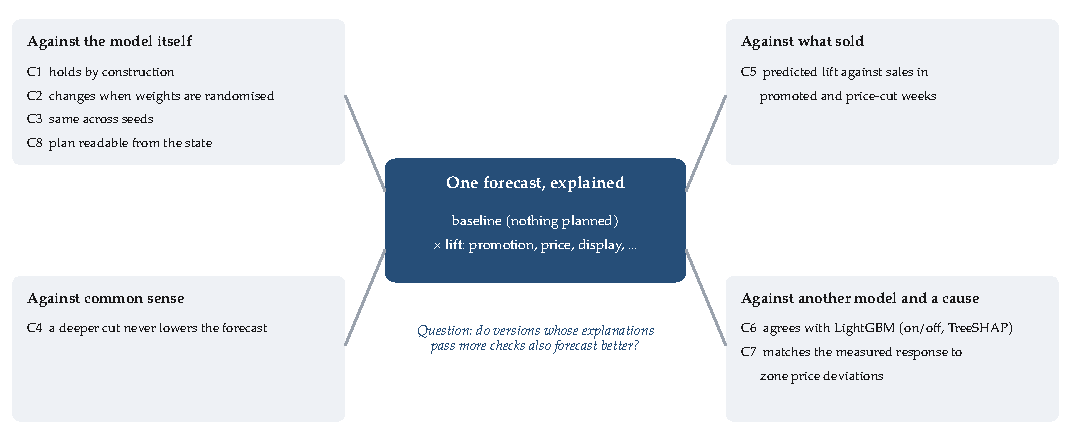
\includegraphics[width=\textwidth]{figs/fig_audit.pdf}
\caption{\textbf{Each forecast's explanation is checked against the model
itself, common sense, what sold, another model and a measured cause.} The eight
checks are fixed in \texttt{docs/PAPER2\_PLAN.md} before any result; every
model version and every check is reported.}
\label{fig:audit}
\end{figure*}
